\documentclass[12pt,letterpaper]{article}
\usepackage[utf8]{inputenc}
\usepackage[spanish, es-tabla]{babel}
\usepackage[version=3]{mhchem}
\usepackage[journal=jacs]{chemstyle}
\usepackage{amsmath}
\usepackage{amsfonts}
\usepackage{amssymb}
\usepackage{makeidx}
\usepackage{xcolor}
\usepackage[stable]{footmisc}
\usepackage[section]{placeins}
\usepackage{listings}
\usepackage{siunitx}
\sisetup{mode=text, output-decimal-marker = {,}, per-mode = symbol, qualifier-mode = phrase, qualifier-phrase = { de }, list-units = brackets, range-units = brackets, range-phrase = --}
\DeclareSIUnit[number-unit-product = \;] \atmosphere{atm}
\DeclareSIUnit[number-unit-product = \;] \pound{lb}
\DeclareSIUnit[number-unit-product = \;] \inch{"}
\DeclareSIUnit[number-unit-product = \;] \foot{ft}
\DeclareSIUnit[number-unit-product = \;] \yard{yd}
\DeclareSIUnit[number-unit-product = \;] \mile{mi}
\DeclareSIUnit[number-unit-product = \;] \pint{pt}
\DeclareSIUnit[number-unit-product = \;] \quart{qt}
\DeclareSIUnit[number-unit-product = \;] \flounce{fl-oz}
\DeclareSIUnit[number-unit-product = \;] \ounce{oz}
\DeclareSIUnit[number-unit-product = \;] \degreeFahrenheit{\SIUnitSymbolDegree F}
\DeclareSIUnit[number-unit-product = \;] \degreeRankine{\SIUnitSymbolDegree R}
\DeclareSIUnit[number-unit-product = \;] \usgallon{galón}
\DeclareSIUnit[number-unit-product = \;] \uma{uma}
\DeclareSIUnit[number-unit-product = \;] \ppm{ppm}
\DeclareSIUnit[number-unit-product = \;] \eqg{eq-g}
\DeclareSIUnit[number-unit-product = \;] \normal{\eqg\per\liter\of{solución}}
\DeclareSIUnit[number-unit-product = \;] \molal{\mole\per\kilo\gram\of{solvente}}
\usepackage{cancel}
\usepackage{graphicx}
\usepackage{lmodern}
\usepackage{fancyhdr}
\usepackage[left=4cm,right=2cm,top=3cm,bottom=3cm]{geometry}

\usepackage[backend=bibtex,style=chem-acs,biblabel=dot]{biblatex}
\addbibresource{ref.bib}

\usepackage{titlesec}
\usepackage{enumitem}
\titleformat*{\section}{\bfseries\large}
\titleformat*{\subsection}{\bfseries\normalsize}
\usepackage{float}
\floatstyle{plaintop}
\newfloat{anexo}{thp}{anx}
\floatname{anexo}{Anexo}
\restylefloat{anexo}
\restylefloat{figure}
\usepackage[margin=10pt,labelfont=bf]{caption}
\usepackage{todonotes}
\usepackage[colorlinks=true, 
            linkcolor = blue,
            urlcolor  = blue,
            citecolor = black,
            anchorcolor = blue]{hyperref}

\begin{document}
\renewcommand{\labelitemi}{$\checkmark$}

\renewcommand{\CancelColor}{\color{red}}

\newcolumntype{L}[1]{>{\raggedright\let\newline\\\arraybackslash}m{#1}}

\newcolumntype{C}[1]{>{\centering\let\newline\\\arraybackslash}m{#1}}

\newcolumntype{R}[1]{>{\raggedleft\let\newline\\\arraybackslash}m{#1}}

\begin{center}
	\textbf{\LARGE{Construção gráfica do software de análise de séries temporais - Um update dos trabalhos desenvolvidos}}\\
	\vspace{7mm}
	\textbf{\large{LaCCAN - Laboratório de computação científica e análise numérica}}\\ 
	\vspace{4mm}
	\textbf{\large{Aluna: Eduarda Chagas}}\\
	\vspace{4mm}
	\textbf{\large{Orientador: Alejandro Frery}}\\
\end{center}

\vspace{7mm}

\section*{\centering Resumo}

Visando relatar os últimos avanços realizados no projeto de pesquisa de implementação do software de análise de séries temporais, tal relatório informa quais funções foram desenvolvidas ao longo do último update discultido, destacando os problemas encontrados e as possíveis soluções a serem abordadas.

Assim, vamos primeiramente descorrer a respeito da ferramenta utilizada nesta etapa do projeto, para logo após expor o que foi desenvolvido no último mês de pesquisa.

\section{Introdução}

Um dos grandes objetivos da pesquisa que se encontra sendo desenvolvida é ampliar a aplicabilidade das técnicas de extração de informações de séries temporais, por meio de uma ferramenta portável e interativa de análise. Por meio disso, foram avaliadas algumas opções de ferramentas de GUI que fosse capaz de suportar as funcionalidades desenvolvidas em \texttt R na primeira etapa.

Como discutido no último encontro da pesquisa a ferramenta de interface gráfica \texttt RGtk2 foi escolhida por atender os pré requisitos discutidos, como:

\begin{itemize}
\item Portabilidade: Deve ser possível implementar o programa de tal modo que este seja executado sem grandes modificações em diferentes sistemas operacionais de desktop.
\item Facilidade de instalação: Como queremos por meio do desenvolvimento do projeto facilitar de um modo geral a análise de séries temporais na experiência do usuário, logo esta não deverá apresentar problemas no processo de instalação.
\end{itemize}

\section{Resultados}

\subsection{Objetivo a ser alcançado}

Sabendo que primeiramente foi desenvolvido um protótipo de tela de como o projeto deveria se encontrar após o seu termínio na GUI \texttt SWING de Java, estamos seguindo tal modelo durante a produção deste novo modelo.

\begin{figure}
  \centering
  \caption{Imagem do protótipo do modelo desenvolvido}
   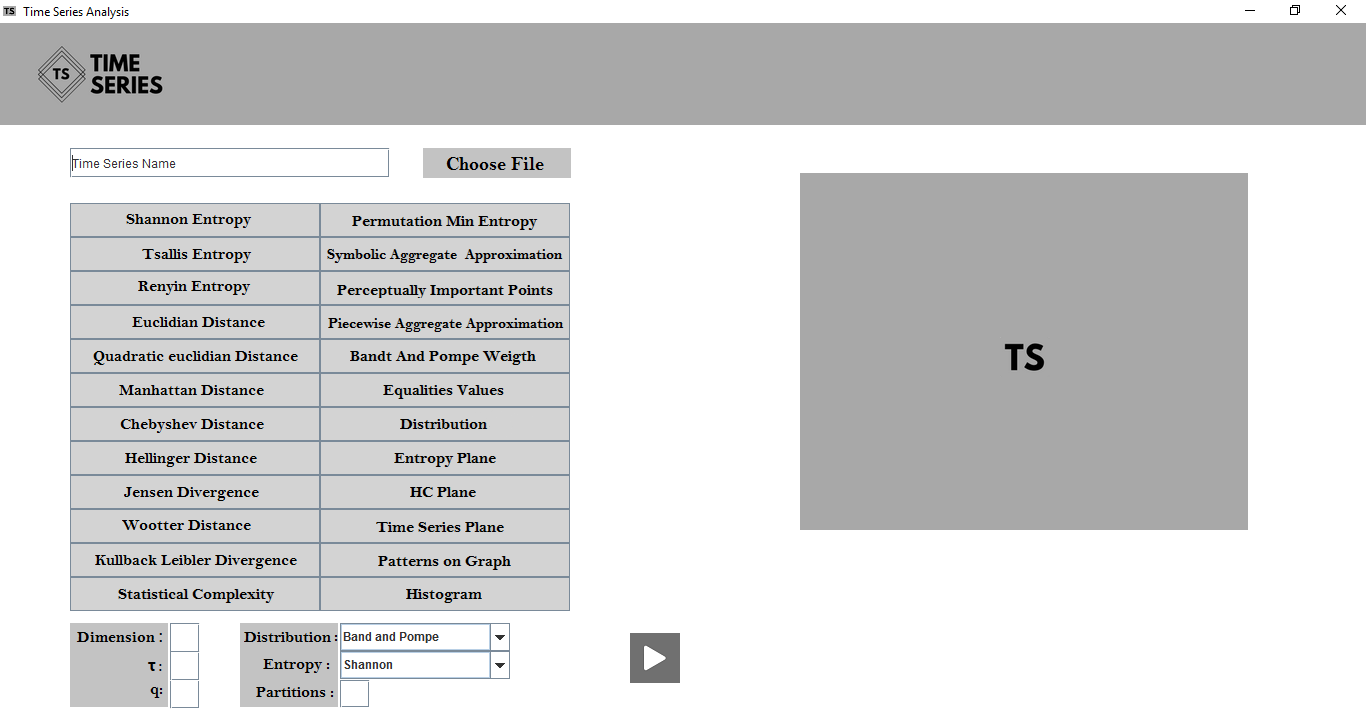
\includegraphics[width=15cm,height=7cm]{tela4.png}
\end{figure}

Logo, o objetivo inicial seria seguir o desenvolvimento utilizando a biblioteca \texttt SWING, no entanto seria necessário a implementação individual do software para cada sistema operacional, já que o programa deveria ser capaz de  reconhecer o sistema utilizado pelo cliente e assim executar seguindo as regras e padrões deste.

\subsection{Resultados reproduzidos até o momento}

Com a troca da ferramenta de interface, podemos perceber que o funcionamento da GUI em \texttt R possui um comportamento bastante diferente da GUI em \texttt Java. Logo, foi necessário primeiramente um estudo de documentações referentes a mesma.

De acordo com \cite{rgtk2} a biblioteca funciona por meio de blocos verticais e horizontais, onde os horizontais se são distribuídos diante dos verticais. Logo foram encontrados os seguintes problemas durante a implementação:

\begin{itemize}
\item Reproduzir o modelo do protótipo onde a área destinada aos gráficos se encontra lado a lado aos botões refentes as funções implementadas.
\item Implementação da função referente a \texttt file.choose em \texttt R: O escopo das variáveis declaradas dentro das funções de tratamento de interrupções é local, logo ainda estamos estudando uma forma de como utilizar o caminho do arquivo para a série temporal nas demais funções do código.
\item Funções de tratamento de interrupção: No momento em que um botão é acionado este é ligado a uma função de tratamento, no entanto como está possui um escopo local das variáveis ( Por exemplo, a função não consegue modificar o valor de uma variável global) e não possui um modo de retornar os valores dessa função devemos então encontrar uma solução para esta problemática.
\item Parte estética do software: Ainda não possuímos uma grande domínio sobre como implemenatar a parte estética utilizando esta biblioteca, logo ainda devemos realizar uma pesquisa mais abrangente sobre tal tópico.
\end{itemize}

\begin{figure}
  \centering
  \caption{Estrutura de organização dos componentes no RGtk2}
   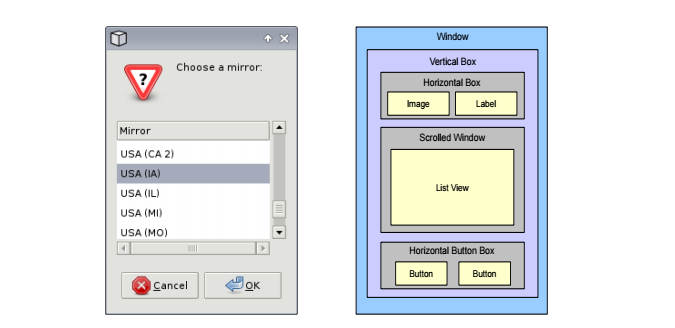
\includegraphics[width=10cm,height=6cm]{estruturaRgtk2.png}
\end{figure}

\begin{figure}
  \centering
  \caption{Modelo reproduzido até o momento com RGtk2}
   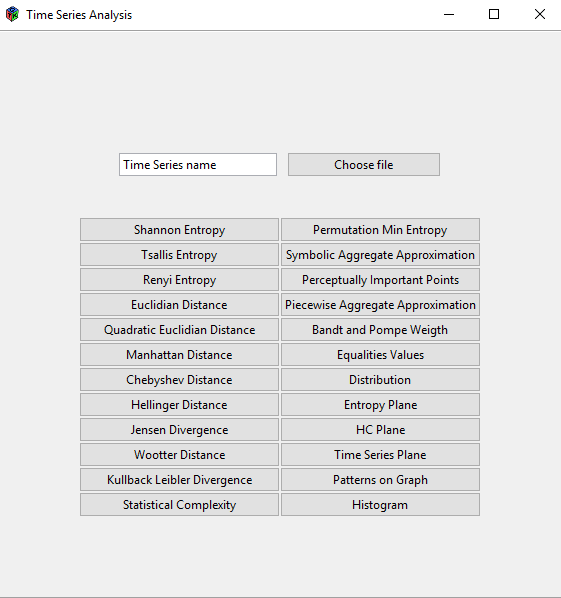
\includegraphics[width=7cm,height=8cm]{modeloRGtk2.png}
\end{figure}

\section{Conclusão}

Desse modo, diante dos problemas identificados possuímos como objetivo solucioná-los até o final do mês presente. E com este relatório visamos atualizar o orientador dos avanços desenvolvidos.


\printbibliography[title=Referências]

\end{document}